\chapter{Part 1}
%• REPORT – Part 1

\section{Introduction}
In this part we discuss the response time analysis of tasks in PU1, PU2 and messages of CAN bus for the configuration given in the assignment. Design and simulation of rotor position and input voltage of DC motor given in the assignment is described. Design space exploration and determining optimal pareto points satisfying design constraints using multi-objective genetic algorithm is discussed.

\section{Response Time analysis}
\subsection{Fixed-Priority Non-Preemptive}
CAN messages follow fixed-priority non-preemptive protocol. The response time analysis for fixed-priority non-preemptive messages can be computed as follows.

\subsubsection{BlockingTime}
Blocking time of a message is defined as the time period for which the message can be blocked by a lower priority message. Therefore blocking time can be computed by finding the maximum of execution of times of all the messages having lower priority than the current message. It can be computed as shown in equation \ref{eq:block}.

\begin{equation}
B_{mi}=\max_{k\epsilon lp(m_i)}(c_i) 
\label{eq:block}
\end{equation}

\subsubsection{BusyPeriod}
Busy Period is defined as the maximum time at which the execution of the message gets completed. It includes the blocking time, delay due to execution of higher priority messages and the message execution time. Busy period of message $m_i$ with priority $i$ can be computed from the equation \ref{eq:busy} with initialization condition shown in equation \ref{eq:init} and termination condition as shown in equation \ref{eq:ter}. 

\begin{equation}
 t_{mi}^{k+1}=B_{mi}+\sum_{\forall m\epsilon hp(m_i)\cup m_i} \lceil{\frac{t_{mi}^k}{p_m}}\rceil c_mi
\label{eq:init}
\end{equation}


\begin{equation}
t_{mi}^0=c_{mi}
\label{eq:ter}
\end{equation}

\begin{equation}
t_{mi}^{k+1}=t_{mi}^{k}
\label{eq:busy}
\end{equation}

\subsubsection{ResponseTime}
If the busy period of the message is less than the period of the message, then the response time of the message is equal to busy period. But if busy period is greater than the period of the message, multiple messages arrive in this instance and response time is computed as the maximum of response times of each individual instances. The number of instances can be computed from equation \ref{eq:inst}. The waiting time and response time of instance $q$ can be computed using equations \ref{eq:wm} and equation \ref{eq:resp} respectively. The initialization and termination conditions for each instance are governed by equations \ref{eq:initw}and \ref{eq:termw} respectively. The total response time can be computed using equation \ref{eq:respfinal}. 

\begin{equation}
Q_{mi}=\lceil \frac{t_{mi}}{p_{mi}}\rceil
\label{eq:inst}
\end{equation}


\begin{equation}
w_{mi}^{k+1}(q)=B_{mi}+qc_{mi}+\sum_{\forall m\epsilon hp(m_i)}\lceil \frac{w_{mi}^k(q)+\tau_bit}{p_{m}}c_m \rceil
\label{eq:wm}
\end{equation}

\begin{equation}
R_{mi}(q)=w_{mi}(q)-qp_{mi}+c_{mi}
\label{eq:resp}
\end{equation}
IniTialization and Termination:

\begin{equation}
w_{mi}^{0}(q)=B_{mi}+qc_{mi}
\label{eq:initw}
\end{equation}

\begin{equation}
w_{mi}^{k+1}(q)=w_{mi}^{k}(q)
\label{eq:termw}
\end{equation}

Total Response time of the message:
\begin{equation}
R_{mi}=\max_{q=0toQ_{mi}}(R_{mi}(q)) 
\label{eq:respfinal}
\end{equation}


\subsection{Fixed-Priority Preemptive}
Unlike the above case messages or tasks can be preempted in Fixed-Priority preemptive case. The processors PU1 and PU2 employ FPP for their task management. The response time of FPP can be calculated as below.
\subsubsection{ResponseTime}
The waiting time and response time of each instance can be calculated from equations \ref{eq:wq} and \ref{eq:rq}. The initialization and termination conditions for each task can be obtained from equations \ref{eq:inw} and \ref{eq:termr}. The response time is nothing but the settling value of the response time.  


\begin{equation}
w_{mi}^{k+1}(q)=w_{mi}^{k}(q)+\sum_{\forall m\epsilon hp(m_i)}\lceil \frac{R_{mi}^k(q)}{p_{m}}c_m \rceil
\label{eq:wq}
\end{equation}

\begin{equation}
R_{mi}(q)=w_{mi}(q)+c_{mi}
\label{eq:rq}
\end{equation}
IniTialization and Termination:

\begin{equation}
w_{mi}^{0}(q)=0;
\label{eq:inw}
\end{equation}

\begin{equation}
R_{mi}^{k+1}(q)=R_{mi}^{k}(q)
\label{eq:termr}
\end{equation}






% Table generated by Excel2LaTeX from sheet 'Sheet1'
\begin{table}[htbp]
	\centering
	\caption{By running the Matlab script ResponsetimeAnylsis\_FPP.m with the different parameters given for PU1 and PU2 these response times are obtained for each of the tasks. These files are then delivered as PU1.m PU2.m}
	\begin{tabular}{rrrrr}
		& & & & \\
		\toprule
		PU1     & $T_1$    & $T_2$    & $T_3$    & $T_4$  $(T_s)$ \\
		\midrule
		Matlab (ms)      & 0.1     & 2.1     & 4.1     & 7.2 \\
		
		& & & & \\
		\toprule
		PU2     & $T_5$    & $T_6$    & $T_7$    & $T_8$ \\
		\midrule
			Matlab (ms)      & 6       & 3       & 9       & 5 \\
		
	\end{tabular}%
	\label{tab:pu-rt}%
\end{table}%




% Table generated by Excel2LaTeX from sheet 'Sheet1'
\begin{table}[htbp]
	\centering
	\caption{Response times for the CAN bus messages}
	\begin{tabular}{rrrrr}
		\toprule
		CAN     & $m_2$   & $m_1$   & $m_3$   & $m_8$ \\
		\midrule
		Matlab (ms) & 2       & 3       & 4       & 4 \\
		
	\end{tabular}%
	\label{tab:can-rt}%
\end{table}%

\section{System Model Derivation and Control Parameter Design}
%• System model derivation, design space exploration and controller
%parameter design
The objectives for the controller is to properly control the given system with a set of design parameters. These parameters, shown in Table %\ref{tab:design}, have to be design and put into perspective with our system, which role they play and the best way to derive them adequately.

There are namely a number of steps taken until all parameters can be considered to satisfy the performance constraints of the controller. These basic steps can be seen in the following list.

\begin{enumerate}
	\item Step 1: Derive the system model. Determine the A, B and C matrices in relation to all constants by hand calculations. We are already provided with the matrices in assignment description, hence no need to derive.Insert this into Matlab.
	 	
	\item Step 2: Derive the values for sampling period and sensor-to-actuator delay based on our system design.
	
	\item Step 3: Choosing desired poles according to the given requirements. Verfiying the controllability of the system for the choosen values. Computing the controller Feed-Forward and Feed-Back gains $F$ and $K$. Inserting these calculations into MATLAB. More about this step can be found in Section %\ref{sec:platform}.
	
	\item Step4: Design K and F values, compute current input activation(u) and outputs(x) from equations, insert these calculations to MATLAB and simulate the system. 
	
	\item Step5: Apply multi-objective genetic algorithm on the above system, with pole positions as parameters, and settling-time and maximum input voltage as our objectives. Obtain pareto optimal points satisfying design constraints. 
\end{enumerate}


	
	\begin{table}[htbp]
		\centering
		\caption{Constants and design parameters referenced to in calculations}
		\begin{tabular}{llll}
			\toprule
			Symbol & Description & Value & Unit\\ 
			\midrule
			$\theta$ & Rotor position  & -&rad \\ 
			$i_m$ & Motor current  & - &A \\ 
			J & Inertia  & $3.2284\cdot10^{-6}$&$Kgm^2$  \\ 
			b & Friction  coefficient   &$ 3.5077\cdot10^{-6} $&Nms/rad\\ 
			R & Armature Resistance  & 4 &Ohm\\
			L & Inductance of Motor Winding  & $2.75\cdot10^{-6}$&H \\ 
			$K_m$ & Motor constant  & $0.0274$&Nm/A  \\ 
			K&Feed-BackGain&-&-\\
			F&Feed-Forward Gain&-&-\\
			\midrule
		\end{tabular}
		\label{tab:constants}
	\end{table}
	
	
	
	\subsection{Controller Structure}
	\label{sec:controllerstructure}
	The system can be described with the second order differential equation shown in Equation \ref{eq:1} as given in the assignment description. Equation \ref{eq:2} and Equation \ref{eq:3} describe the statespace representation of our system. From these equations the Feedback- and Feedforward gain can be determined in relations to the constants in the system. 
	
	
	\begin{equation}
	\text{\textit{\textbf{x}}} =
	\begin{bmatrix}
	x_1 \\
	x_2  \\
	x_3   
	\end{bmatrix}
	=
	\begin{bmatrix}
	\theta\\
	\dot{\theta}\\
	i
	\end{bmatrix}
	=
	\begin{bmatrix}
	\theta\\
	\omega\\
     i
	\end{bmatrix}
	\quad\text{ and }\quad
	\dot{\text{\textit{\textbf{x}}}} =
	\begin{bmatrix}
	\dot{\theta}\\
	\ddot{\theta}\\
	\dot{i}
	\end{bmatrix}
	\vspace{.2em}
	\label{eq:1}
	\end{equation}
	

	
	\begin{equation}
	\dot{\text{\textit{\textbf{x}}}}  = {\text{\textbf{A}}}\text{\textit{\textbf{x}}}  +  {\text{\textbf{B}}}\text{\textit{{u}}}  \text{ and } \text{\textit{{y}}}  = {\text{\textbf{C}}}\text{\textit{\textbf{x}}}  \qquad \text{ where } \quad \text{input: \textit{{u}}}=V \quad\text{ , output: \textit{{y}}}=i
	\label{eq:2}
	\end{equation}
	
	%Equation \ref{eq:4} and \ref{eq:5} show the same equation. But the matrices can be derived by combing the equations above and resulting in Equation \ref{eq:5}. This can then be used to calculate the K and F values mentioned in Table \ref{tab:design}.
	
	\begin{equation}
	\dot{\text{\textit{\textbf{x}}}}  = \begin{bmatrix}
	0 & 1 & 0 \\
	0&\frac{-b}{J}&\frac{K_m}{J} \\
	0&\frac{-K_m}{L}&\frac{-R}{L} \\
	\end{bmatrix}
	\begin{bmatrix}
	\theta\\
	\omega\\
	i\\
	\end{bmatrix}
	+
	\begin{bmatrix}
	0\\
	0\\
	\dfrac{1}{L}\\
	
	\end{bmatrix}\text{\textit{{V}}}
	\quad \text{ and } \quad
	\text{\textit{{y}}}=\begin{bmatrix}
	1&0&0
	\end{bmatrix}
	\begin{bmatrix}
	\theta\\
	\omega\\
	i\\
	\end{bmatrix}
	\label{eq:3}
	\end{equation}
\subsection{Controller Design}
In this subsection we discuss the method for designing the controller design parameters FeedbackGain-$K$ and FeedForwardGain-$F$. In this problem we have the scenario where $D_c<h$. Since our controller operates in discrete sample time, we start with converting our continuous system as described in equation \ref{eq:code1} into discrete domain. Therefore on applying ZOH sampling with period $h_c$ and constant sensor-actuator Delay $D_c$ we achieve the equation \ref{eq:code2} for discrete sample time system. From \ref{eq:code2} we can notice that the next output not only depends on current input but also on previous input. Hence, we simplify the system and get it into standard form representing equation \ref{eq:code3} by invoking equation\ref{eq:code6}. After applying above simplification input $u[k]$ can be represented in terms of controller gains using equation\ref{eq:code7}. 
and matrices $\Phi$ ,$C$ are converted to corresponding augmented matrices $\Phi_{aug}$,$C_{aug}$, whereas $\Gamma_1$,$\Gamma_2$ are converted to single augmented matrix $\Gamma_{aug}$.
\begin{equation}
\dot{x}  =  A x  +   B u  \quad{\text{   and   } }\quad  y  =  C x  
\label{eq:code1}
\end{equation}


\begin{equation}
x[k+1]= \phi x [k]+ \Gamma_1(D_c)u[k-1]+\Gamma_0(D_c)u[k] \quad \text{ and } \quad y[k] = C x[k]
\label{eq:code2}
\end{equation}


\begin{equation}
x[k+1]= \phi z [k]+ \Gamma_{aug}u[k] \quad \text{ and } \quad y[k] + C_{aug} z[k]
\label{eq:code3}
\end{equation}

\begin{equation}
z[k]=\begin{bmatrix}
x[k]\\
u[k-1]
\end{bmatrix}
\label{eq:code6}
\end{equation}

\begin{equation}
u[k] = Kz[k] + Fr 
\label{eq:code7} 
\end{equation}


\begin{equation}
 K = -[ \ 0 \ 0 \ \cdots \ 1 \ ] \gamma_{aug}^{-1} H(\phi_{aug})
\label{eq:code4} 
\end{equation}

\begin{equation}
 F = \dfrac{1}{C_{aug} (I-\phi_{aug}-\Gamma_{aug}K)^{-1}\Gamma_{aug}}
\label{eq:code5}
\end{equation}



Before deriving the controller gains it is important to verify if the system is controllable under given configuration. This can be verified by calculating $det(\gamma_{aug})$. If the determinent is not equal to 0, then system is controllable. After verifying the controllability of the system $K$ can be derived by applying Ackermanns formula described in equation \ref{eq:code4} and $F$ can be derived from equation \ref{eq:code5} . However, one can notice the matrix $H(\Phi_{aug})$ depends on the desired poles which in turn depends on the design requirements. The desired poles alter the frequency spectrum of the transfer function of the system and play a significant role in controlling the behavariour of output parameters of the system. Therefore various design requirements such as Overshooot, settling time, boundary ranges of the parameters in the system depends on the desired poles and thus in turn influence controller gains $K$ and $F$. Following design, work flow has been developed in MATLAB to derive pareto optimal points(pole locations) satisfying design constraints using multi-objective genetic algorithm and one of the optimal point is selected for simluation.


\section{Simulation and Design Decisions}
Foll0wing are the design decisions taken before simulating the system.

\begin{enumerate}
\item Employing Rate-Monotonic -Scheduling (RMS). That is the tasks with lower period gets higher priority. This ensures Task $T_s$ and message $m_s$ have highest priorities and thus reducing sensor-actuator delay. Therefore Sensor-to-actuator delay can be computed as 
$$D_c=T_s+m_s+2S+T_ca$$ This results in sensor-to-actuator delay of 8.1ms.
The TDMA cycle of PU3 is 10ms$(>D_c)$. Therefore we can have a sampling period of 10ms.
\item Simulate the above system using above design parmeters $h_c$ and $D_c$.Apply multi-objective genetic algorithm on the above system, with pole positions as parameters, and settling-time and maximum input voltage as our objectives. The design constraints are settling time less than 400ms and input voltage less than 1v. Obtain pareto optimal points satisfying design constraints.  The lower and upper bounds used for pole positions are 0 and 1 respectively.
\end{enumerate}
%• Your design decision and justification.

\section{Results}
%• Results
The input data (period, deadline ,wcet and priority) for both the processors and CAN bus is shown in the left part of the figure \ref{fig:inchronprios}. The priorities for tasks are chosen according to Rate-Monotonic-Scheduling (RMS).  The simulation for response times for PU1 and PU2 is computed using $'ResponseTimeAnanlysis\_FPP.m'$ which performs the calculations shown described in section 1.2.2 while the response time for CAN bus is computed using $'ResponseTimeAnanlysis\_FPNP.m'$ which performs the calculations shown described in section 1.2.2. The response times for tasks in PU1 and PU2 are shown in Table \ref{tab:pu-rt} and the response time of CAN messages is shown in Table \ref{tab:can-rt}. The pareto front and the score histogram for optimal pole positions is shown in figure \ref{fig:pareto}. The pareto optimal points are presented in Table \ref{tab:pareto}. The middle point is taken for simulation and the plots for rotor position and input voltage are shown in figure \ref{fig:rv}.
\begin{figure}[h!]
	\begin{center}
		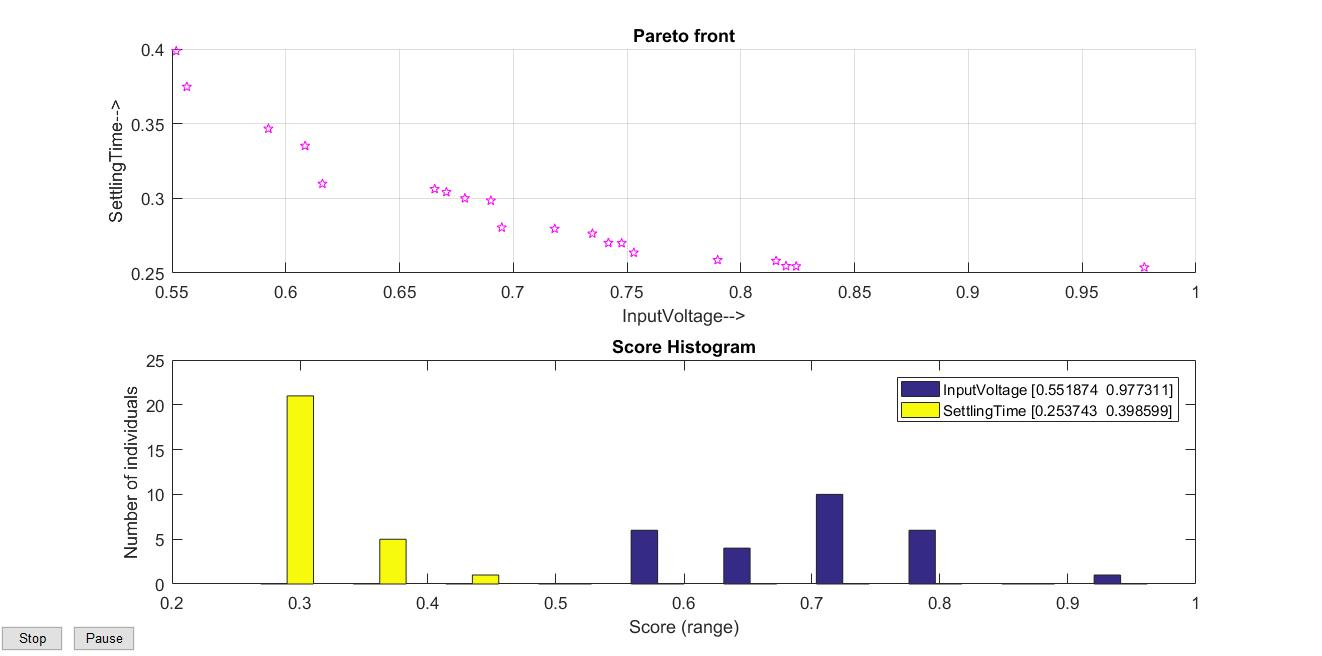
\includegraphics[width=\linewidth]{img/pareto}
		\caption{Pareto Plot and score histogram for various pole positions with settling time and input voltage as objectives}
		\label{fig:pareto}
	\end{center}
\end{figure}

\begin{figure}[h!]
	\begin{center}
		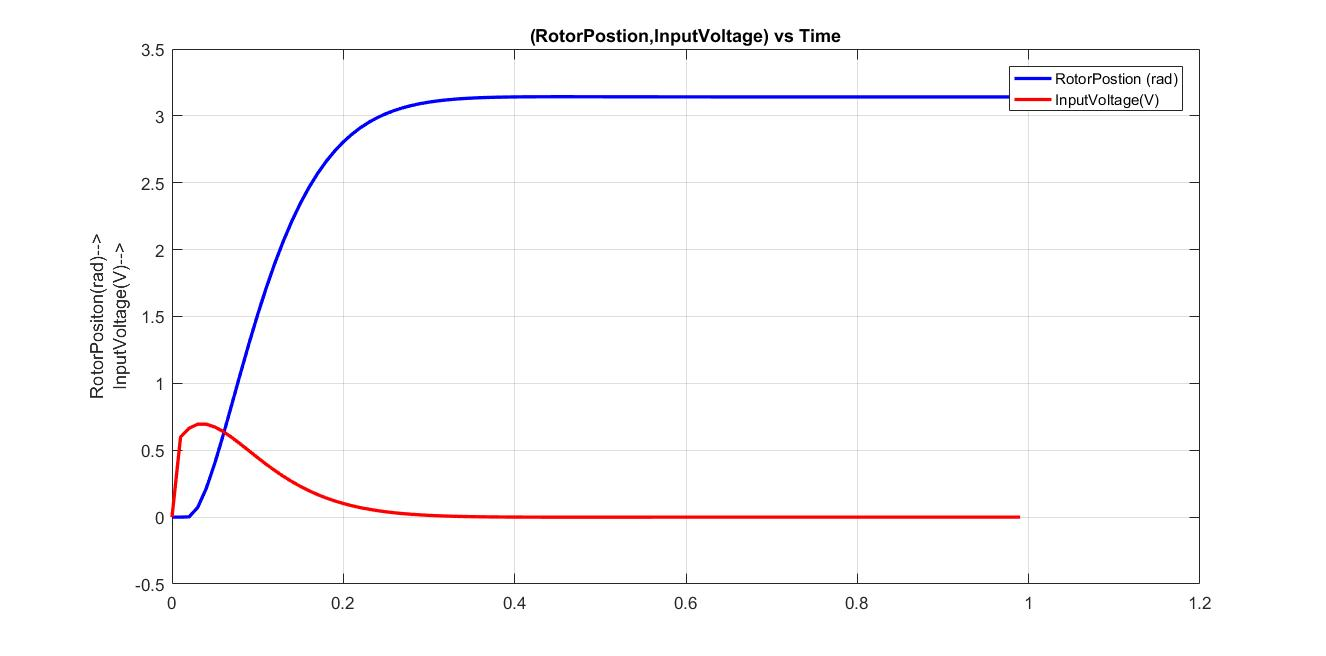
\includegraphics[width=\linewidth]{img/rv}
		\caption{Change in Rotor Position and Input Voltage with time (for the 10th pareto point)}
		\label{fig:rv}
	\end{center}
\end{figure}

\begin{table}[]
	\centering
	\label{tab:pareto}
% Please add the following required packages to your document preamble:
% \usepackage{booktabs}

	
		\begin{tabular}{|l|l|l|l|l|l|}
			\hline
			InputVoltage(V) & SettlingTime(sec) & P1        & P2      & P3      & P4        \\ \hline
			0.55187         & 0.3986            & 0.042356  & 0.79712 & 0.86895 & 0.032116  \\ \hline
			0.55651         & 0.37465           & 0.033305  & 0.79853 & 0.87171 & 0.039792  \\ \hline
			0.59234         & 0.34662           & 0.0058031 & 0.82007 & 0.84669 & 0.036008  \\ \hline
			0.60848         & 0.33514           & 0.036173  & 0.79947 & 0.85949 & 0.032497  \\ \hline
			0.6161          & 0.30976           & 0.019745  & 0.82096 & 0.84783 & 0.029296  \\ \hline
			0.66542         & 0.30623           & 0.043944  & 0.79782 & 0.83793 & 0.01936   \\ \hline
			0.67059         & 0.30415           & 0.02643   & 0.80271 & 0.83055 & 0.023413  \\ \hline
			0.6787          & 0.3               & 0.019514  & 0.80909 & 0.82646 & 0.01884   \\ \hline
			0.6901          & 0.2985            & 0.026171  & 0.80598 & 0.82174 & 0.018069  \\ \hline
			0.69489         & 0.28047           & 0.023082  & 0.80557 & 0.82825 & 0.02835   \\ \hline
			0.71815         & 0.27962           & 0.017678  & 0.80943 & 0.81624 & 0.0096658 \\ \hline
			0.73472         & 0.2764            & 0.026266  & 0.79633 & 0.82358 & 0.017902  \\ \hline
			0.74179         & 0.27011           & 0.030858  & 0.80199 & 0.81578 & 0.015076  \\ \hline
			0.7476          & 0.26996           & 0.019604  & 0.79668 & 0.81833 & 0.0062062 \\ \hline
			0.75291         & 0.26361           & 0.023345  & 0.79621 & 0.81719 & 0.028087  \\ \hline
			0.78977         & 0.25864           & 0.027588  & 0.79019 & 0.80703 & 0.020728  \\ \hline
			0.81545         & 0.25809           & 0.020387  & 0.7722  & 0.81093 & 0.033555  \\ \hline
			0.81984         & 0.25468           & 0.0095985 & 0.79821 & 0.7961  & 0.013229  \\ \hline
			0.8243          & 0.25444           & 0.010459  & 0.7929  & 0.79613 & 0.013602  \\ \hline
			0.97731         & 0.25374           & 0.012836  & 0.78696 & 0.75179 & 0.024935  \\ \hline
		\end{tabular}


\caption{Pareto Points (Pole locations) for Input Voltage and Settling Time}

\end{table}










%• 3 processors:
%• PU1: Fixed Priority Preemptive (FPP)
%• PU2: Fixed Priority Preemptive (FPP)
%• PU3: CompSOC platform using Time Division Multiplexing (TDM) with a clock
%frequency running @ 100 MHz
%− Partition slots: 245904 clock cycles: 2.45904 ms
%− CoMik slots: 4096 clock cycles: 40.96 us
%− TDM period: 1000000 clock cycles: 10 ms
%− 4 Partition slots, 4 CoMik slots
%• Multiple tasks running on each processor
%• PU1: T1, T2, T3, Ts
%• PU2: T5, T6, T7, T8
%• PU3: S1 (unassigned), S2 (T4), S3 (Tca), S4 (unassigned)
%• Communication task in all processors has a WCETcom = 0.05 ms
%• Communication bus : CAN
%• Transmission of each message over the CAN bus takes 1 ms

%
%• Design the controller and its implementation such that
%1. The real-time tasks meet their deadlines and end-to-end delay
%requirements. For this assign the priorities in each processor
%and the CAN bus to meet the requirements. You may use the
%response time analysis MATLAB scripts provided with the
%assignment.
%2. Input signal 𝐕𝐕 should be designed such that the motor position
%(shatft angle) is 𝜽𝜽 = 𝟑𝟑. 𝟏𝟏𝟏𝟏𝟏𝟏𝟏𝟏 rad for a maximum available input
%signal is 1 V, and maximum settling time of 400 ms
%3. A design space exploration of system poles which satisfy the
%requirements (input signal, settling time) should be done.
%4. Hint: use the sampled-data model used in the lectures (derive
%the augmented system). Be careful during discretization.

%• Response time analysis processor PU1 (PU1.m)
%• Response time analysis processor PU2 (PU2.m)
%• Response time analysis for CAN messages (CAN.m)
%• Control design and simulation (Control_p1.m)
%• A PDF report (a2.pdf)
%• See details of the report later